%%%%%%%%%%%%%%%%%%%%%%%%%%%%%%%%%%%%%%%%%%%%%%%%%%%%%%%%%%%%%%%%%%%%%%%%%%%%%%%%%%%%%%%%%%%%%%%%%%%%%%%%%%%%%%%%%%%%%%%%%%%%%%%%%%%%%%%%
% This is just a template to use when submitting manuscripts to Frontiers, it is not mandatory to use frontiers.cls nor frontiers.tex  %
%%%%%%%%%%%%%%%%%%%%%%%%%%%%%%%%%%%%%%%%%%%%%%%%%%%%%%%%%%%%%%%%%%%%%%%%%%%%%%%%%%%%%%%%%%%%%%%%%%%%%%%%%%%%%%%%%%%%%%%%%%%%%%%%%%%%%%%%

\documentclass{frontiersSCNS} % for Science articles
%\documentclass{frontiersMED} % for Medicine articles

\usepackage{url}

%\usepackage{lineno}
\usepackage{todonotes}
\usepackage{listings}
\lstset{language=Python}

\newcommand{\alex}[1]{\todo[inline, color=green!40]{#1}}
\newcommand{\fabian}[1]{\todo[inline, color=blue!40]{#1}}



%\linenumbers


\copyrightyear{}
\pubyear{}
%\onecolumn
%%% write here for which journal %%%
\def\journal{Neurosciences}
\def\DOI{}
\def\articleType{}
\def\citing{\color{darkgray}\cite}
\def\keyFont{\fontsize{6}{11}\helveticabold }
\def\firstAuthorLast{Alexandre Abraham {et~al}} %use et al only if is more than 1 author

% XXX Review the order of authors

\def\Authors{Alexandre Abraham\,$^{1,2,*}$, Philippe Gervais\,$^{1,2}$, Fabian
Pedregosa\,$^{1,2}$, Andreas Muller, Jean Kossaifi, Michael Eickenberg, Alexandre Gramfort, Bertrand
Thirion\,$^{1,2}$ and Ga\"el Varoquaux\,$^{1,2}$}
% Affiliations should be keyed to the author's name with superscript numbers and be listed as follows: Laboratory, Institute, Department, Organization, City, State abbreviation (USA, Canada, Australia), and Country (without detailed address information such as city zip codes or street names).
% If one of the authors has a change of address, list the new address below the correspondence details using a superscript symbol and use the same symbol to indicate the author in the author list.
\def\Address{
    $^{1}$Parietal Team, INRIA Saclay-\^{I}le-de-France, Saclay, France\\
    $^{2}$Neurospin, I\textsuperscript{2}BM, DSV, CEA, 91191 Gif-Sur-Yvette, France}

% The Corresponding Author should be marked with an asterisk
% Provide the exact contact address (this time including street name and city zip code) and email of the corresponding author
\def\corrAuthor{Alexandre Abraham}
\def\corrAddress{Parietal Team, INRIA Saclay-\^{I}le-de-France, Saclay, France}
\def\corrEmail{alexandre.abraham@inria.fr}

% \color{FrontiersBlue} Is the blue color, used in the Journal name, in the title, and the names of the sections


% Example of table from template

% \begin{table}[!t]
% \processtable{Resolution Requirements for the figures\label{Tab:01}}
% {\begin{tabular}{lllll}\toprule
% Image Type & Description & Format & Color Mode & Resolution\\\midrule
% Line Art & An image composed of lines and text,  & TIFF, EPS, JPEG & RGB, Bitmap & 900 - 1200 dpi\\
%            & which does not contain tonal or shaded areas.& & &\\
%            Halftone & A continuous tone photograph, which contains no text. & TIFF, EPS, JPEG & RGB, Grayscale & 300 dpi\\
% Combination & Image contains halftone + text or line art elements. & TIFF, EPS, JPEG & RGB,Grayscale & 600 - 900 dpi\\\botrule
% \end{tabular}}{This is a footnote}
% \end{table}


% Figures

% \textbf{Figure 1.}{ Enter the caption for your figure here.  Repeat as  necessary for each of your figures.}\label{fig:01}
% Don't add the figures in the LaTeX files, please upload them when submitting the article. Frontiers will add the figures at the end of the provisional pdf.



\begin{document}
\onecolumn
\firstpage{1}

\title[Machine Learning for Neuroimaging with Scikit-Learn]{Machine Learning for Neuroimaging with Scikit-Learn}
\author[\firstAuthorLast ]{\Authors}
\address{}
\correspondance{}
\editor{}
\topic{Research Topic}

\maketitle
\begin{abstract}

\section{}
Statistical learning methods are increasingly used to perform
neuroimaging analysis. Their main virtue for this type of application
is their ability to model high-dimensional datasets, e.g.\ multivariate
analysis of activation images, or capturing inter-subject variability.
Supervised learning is typically used in “decoding” setting to relate
brain images to behavioral or clinical observations, while
unsupervised learning is typically used to uncover hidden structure in
sets of images (e.g.\ resting state functional MRI) or to find
sub-populations in large cohorts of subjects. By considering
functional neuroimaging use cases, we illustrate how scikit-learn,
a Python machine learning library, can be used to perform some key
analysis steps. Scikit-learn contains a large set of statistical
learning algorithms, both supervised and unsupervised, that can be applied
to neuroimaging data after a proper preprocessing. Combined with other
Python libraries, neuroimaging data can be loaded, processed and the results
can be visualised easily.



\tiny
% XXX Fix keywords
%All article types: you may provide up to 8 keywords; at least 5 are mandatory.
\section{Keywords:} machine learning, statistical learning, neuroimaging, scikit-learn, python
\end{abstract}


\section{Introduction}

Python is being increasingly used in neuroimaging studies, \cite{millman2007analysis, hanke2009pymvpa}, which can be explained its
versatility, its ability to act as a glue between different components and the
maturity of its scientific stack.


\subsection{Scientific Python and neuroimaging ecosystem}

\subsubsection{Scipy and Numpy}

SciPy and NumPy packages are the basis of scientific computing in Python.
NumPy provides the \verb!ndarray! data type, an efficient $n$-dimensional data
representation. These vectors holds all common operations (transpose...) and
can be easily manipulated thanks to a simple, yet powerful, indexing. SciPy
provides higher level mathematical functions that operate on ndarrays for a
variety of domains including linear algebra, optimization and signal
processing. Together, NumPy and SciPy provide a robust scientific environment
for numerical computing and they are the elementary bricks we use in all our
algorithms.

\subsubsection{matplotlib}

Matplotlib is a Python plotting library that is tightly integrated into the
rest of the scientific python stack. It offers publication quality figures in
a variety of formats and allows to display plots, images or 3D plots in a
graphical user interface. All figures in this paper have been generated using
this library.


\subsubsection{nibabel}

Nibabel is a neuroimaging data loading package. Nibabel can load or save data in
the most popular neuroimaging data format. This is indeed an entry point of all
our scripts.

\subsubsection{nipy}


\subsubsection{scikit-learn}

The {\em scikit-learn} project, \cite{pedregosa2011}, is an open source machine
learning library for the Python programming language. The ambition of the
project is to provide efficient and well-established machine learning tools within
a programming environment that is accessible to non-machine learning experts
and reusable in various scientific areas.



% Here we present the Python neuroimaging ecosystem : scikit­learn, nibabel,
% nipy.

\section{Scikit-learn concepts}

% Present the underlying concepts of scikit­learn: estimator,­ data
% representation, transformer...

All objects within \sklearn share a uniform common basic API consisting of three
complementary interfaces: an \textit{estimator} interface for building and
fitting models, a \textit{predictor} interface for making predictions and a
\textit{transformer} interface for converting data into a different representation.

Interoperation with third-party code is made not on base on inheriting from a
particular class but on the base of implementing the appropriate methods for a
given interface.

\subsection{Estimator}

The \textit{estimator} interface is at the core of the library. It exposes a
\texttt{fit} method for learning a model from training data.  All supervised
and unsupervised learning algorithms (e.g., for classification, regression or
clustering) are offered as objects implementing this interface. Machine
learning tasks like feature extraction, feature selection or dimensionality
reduction are also provided as estimators.

\subsection{Predictor}

The \textit{predictor} interface extends the notion of an estimator
by adding a \texttt{predict}
method that takes an array \texttt{X\_test} and produces
predictions for \texttt{X\_test}, based on the learned parameters of the
estimator (we call the input to \texttt{predict} ``\texttt{X\_test}'' in order
to emphasize that \texttt{predict} generalizes to new data). In the case of
supervised learning estimators, this method typically returns the predicted
labels or values computed by the model.

\subsection{Transformer}


\subsection{Data representation}

In the scikit learn, and in the world of statistical machine learning, data are
usually represented in a 2-dimensional matrix of shape $n\_samples \times
n\_features$. 


A tranformer is an object that exposes a \verb!transform! method. If the transformation
can be inverted, a method called \verb!inverse_transform! also exists.


\subsection{Cross validation}

\alex{It seems more right to me to put it in this part}


\section{From MR volumes to a data matrix}

As any domain specific data, MR volumes holds particular properties.
Understanding them is crucial to be sure to make proper use of the data.

\[
    \begin{bmatrix}
        r_x & 0   & 0   & o_x \\
        0   & r_y & 0   & o_y \\
        0   & 0   & r_z & o_z \\
        0   & 0   & 0   & 1   \\
    \end{bmatrix}
    \begin{bmatrix}
        x \\
        y \\
        z \\
        1 \\
    \end{bmatrix}
\]

\subsection{Data Preparation}
    % or Signal Processing ?

At this point, we suppose that standard preprocessings have been applied to the
data. They should be registrated on a common template (MNI for example).
However, data is not yet ready to be processed by the scikit-learn. In
fact, preprocessed data may have different shapes. Moreover, it is essential to
get rid of some remaining scanner artefacts and individual trends.

\subsubsection{Detrending}

Detrending is an essential step when dealing with fMRI data. It removes a
best-fit linear trend (in the least square sense) over the time series of each
voxel. It is obviously needed when you want to study the correlation between
features.

\begin{lstlisting}
scipy.signal.detrend(data)
\end{lstlisting}

\alex{Gaël told me not to go deep into the maths, I wonder if talking about
      least squares is a good idea. Maybe I should say that a constant trend is a
      mean and a linear trend is simply a linear function}

\subsection{Resampling}

Resampling consists in changing the shape of the data. This is typically needed
when dealing when data coming from an heterogenous dataset, as the shape depends
on acquisition parameters.

Practically, resampling is an interpolation and thus may alterate the integrity
of the data. That is why it should be used carefully. Oversampling (increasing
data resolution) leads to higher memory consumption and computation resources.
Downsampling is commonly used to reduce the size of the data we want to process.

Typical sizes are 2mm or 3mm resolutions, but the spread of high field MR
scanner tends to lower these values.

\subsection{Signal cleaning}

\begin{itemize}
    \item Remove high frequency (scanner artefacts)
    \item Removing confounds is necessary for some treatments
\end{itemize}


% I think that we should present the challenges about NI data here. Poor SNR,
% multi subject / session...

\subsection{Masking}

% This   step  turns  the  data  into  the  scikit­learn   compliant  formant
% n_features  x  n_samples.  We  may speak of connectivity graph that allow to
% integrate the 3D structure of the data in some algorithms.

\subsubsection{From 4-dimensional image to 2-dimensional array}

Neuroimaging data are represented in 4 dimensions: 3 dimensions for the scans,
which are positioned in a coordinate space, and one dimension for the time.
Scikit-learn algorithms, on the other hand, only accept 2-dimensional data: one
dimension for the features and one for the samples.\\

Consequently, in order to use neuroimaging data in the scikit-learn, a
conversion is needed. The most simple way to achieve that would be to
\emph{flatten} the 3D scans into a 1D array. However, we know that not every
voxels in a neuroimaging scan is useful. In particular, outter-brain voxels are
of no use and, worse, they can bring spurious noise and scanner artefacts (such
as ghosts).\\

To sort out voxels of interest, we will have to apply a mask on the data. Most
of public datasets provide a mask, come of them even provide several, isolating
different functional or anatomical brain regions. \alex{ref to Haxby}

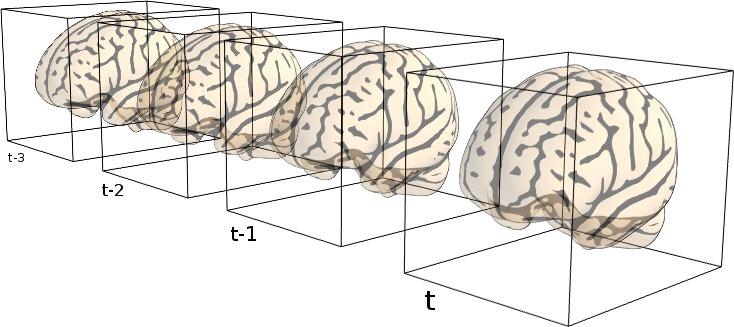
\includegraphics[width=.5\linewidth]{img/niimgs.jpg}

\alex{Should tell here that some algorithms, like logistic regression, do not
like colinear features.}

\subsubsection{Automatically computing a mask}

The simplest strategy to compute a mask is a binarization by a selected threshold.
Due to the nature of the neuroimaging data, there exists some strategy to choose
this threshold in order to obtain a decent segmentation.

\alex{There is a reference for the method used in Nisl. We should put it there
and in the code. Add a figure with an histogram to illustrate.}

Multi subject computation is simply done by intersecting subjects maps
relatively to a chose threshold.

\subsubsection{Conserving geometrical structure}

Applying a mask on the data obviously remove the 3-dimensional structure of the
data. However, some algorithms, like the Ward, need this structural information.
\verb!sklearn.feature_extraction.image! provides two methods that builds an
adjacency matrix based upon your data while taking the mask into account:
\begin{itemize}
    \item \verb!grid_to_graph! creates a binary adjacency graph based upon the
        data shape. This is useful for Ward's clustering.
    \item \verb!grid_to_graph! creates a distance matrix using the gradient of
        the image. This graph can be used in Spectral clustering.
\end{itemize}

\subsection{Label shifting}

Functional MRI measures brain activity by using the Blood-Oxygen-Level-Dependent
contrast (BOLD). In fact, like muscles, brain regions consumes more oxygen and
nutriments when stimulated. So when a part of the brain starts working,
physiological mechanisms induce an oxygen-rich blood flood toward this
particular region: this is called haemodynamic response.

However, this reaction takes time, usually around 6 seconds. This is the
duration between the event and the reaction observed in the brain. To be able to
match these two events, we will sometimes have to shift our data. The number of
scans taht must be shifted depends on the TR (repetition time) of the data.
Usually, we remove the two first scans of the data and the two last values of the
labels (to keep an homogeneous length).

\begin{lstlisting}
data = data[2:]
labels = labels[:-2]
\end{lstlisting}

\section{Decoding}

The process of predicting behavioral or comportamental data from fMRI scan is
called decoding.


\subsection{SVM}



\subsubsection{Haxby dataset}

For this example and the following, we will use Haxby dataset
(\cite{haxby2001}).
Haxby dataset is from a study about face and object representation into the
brain (in particular in high level visual cortex). It is composed of 12 runs for
each of the 6 subjects. Greyscale images representing faces, houses, cats,
bottles, scissors, shoes, chairs and random textured were presented in 24
seconds blocks separated by rest periods. The repetition time (TR) between each
scan is 2.5s. Full acquisition information are available in the reference paper.

To make this example easier, we will work on a subset of this dataset. We will
consider only one subject and will try to classify faces versus houses.

\subsubsection{Feature selection: ANOVA F-Test}

Even if the resolution of brain-imaging data seems low (3mm cubes, around 100000
neurones), from a computational point of view, this is a huge. For example,
Haxby dataset has a resolution of $64\times64\times40 = 163840\text{ voxels}$.
After applying the mask, only 39912 voxels are left, which is still high.

In order to reduce the number of features, we can aggregate them (in regions of
interest for example) or we can select only the most relevant ones (those who
correlates most with the task). As we expect a lot of feature to be irrelevant
for our task, we opt for a feature selection method.

In supervised learning, the most popular feature selection method is the
ANalysis Of VAriance (ANOVA) F-Test. This is a generalization of the t-test to
more than 2 features. Basically, ANOVA compares several
groups to determine if they are similar (ie randomly drawn form the same
population, this is the null hypothesis). We use it to compare the distributions
of the features values across the classes.

\verb!sklearn.feature_selection! contains a panel of feature selection
strategies. One can choose to take a percentile of the features
(\verb!SelectPercentile!), or a fixed number of features (\verb!SelectKBest!)
for example. All these objects are implemented as transformers.
Here we use a fixed number of features and we use the \verb!f_calssif! function
(ANOVA F-Test) for scoring.

\begin{lstlisting}
from sklearn.feature_selection import SelectKBest, f_classif

### Define the dimension reduction to be used.
# Here we use a classical univariate feature selection based on F-test,
# namely Anova. We set the number of features to be selected to 500
feature_selection = SelectKBest(f_classif, k=500)
\end{lstlisting}

\subsubsection{Support Vector Classifier}

A Support Vector Classifier (SVC) is a simple classifier that finds a linear
hyperplane that separates the samples. Classifying a new example boils down to
seeing on which side of the hyperplane the example is. SVC has the advantage to
give reliable results even when the number of dimensions is greater than the
number of samples.

The decision is taken based upon a subset of training data called support
vectors. We can say that these support vectors holds the information allowing to
discriminate the two classes, this is why we will display them and try to see if
they match some neuroscientific knowledge.

\begin{lstlisting}
from sklearn.svm import SVC
clf = SVC(kernel='linear', C=1.)

### Look at the discriminating weights
svc = clf.support_vectors_
# reverse feature selection
svc = feature_selection.inverse_transform(svc)
\end{lstlisting}

\subsubsection{Pipeline}

The workflow described above (feature selection + estimator) is a standard one.
In fact, in most cases, the workflow will consist in atomic steps
\textit{linked} together (the output of a step is the input of the next one).
For this purpose, scikit-learn offers a pipeline object that allows such
linking. A pipeline is simply a list of scikit-learn objects through which the
input data will be conveyed. The function to call for each object (transform,
fit...) depends on its type.
This allow the developpers to write a complete processing as a one-liner.

\begin{lstlisting}
from sklearn.pipeline import Pipeline
anova_svc = Pipeline([('anova', feature_selection), ('svc', clf)])
\end{lstlisting}

\subsubsection{Displaying the results}
~\\
\alex{Should we define a visualization function once and for all?}

\subsection{Searchlight}

\begin{itemize}
    \item Present the Searchlight problem
    \item Say it is less a pain to implement thanks to scikit-learn bricks
        (estimator and cross\_val). Plus it is easily customizable.
\end{itemize}

\subsection{Classification of M/EEG sensor space data}


\subsection{Orthogonal Matching Pursuit}

\subsubsection{Kamitani dataset}

Kamitani dataset is based on a visual task like Haxby. In this experiment,
several series of $10\times10$ binary images are presented to two subjects.
Our goal will be to use the scikit-learn to learn a correlation between brain
activation and voxel color. Full details are available in the reference paper
(\cite{miyawaki2008}).

Kamitani training set is composed of random images (where black and white pixels
are balanced). The testing set is composed of structured images containing
geometric shape (square, cross...) and letters (spelling the word \emph{neuro}).

There are two ways to establish a link between brain voxels and image pixels: we
can either try to reconstruct image from brain voxel activation, this is called
decoding, or we can try to predict brain activation from an image, this is called
encoding.

In the present example, we will do both encoding and decoding and see if the
results match.

\subsubsection{Preprocessing}

Common pre-treatment have been applied to the data (detrending and
standardization).

\subsubsection{Decoding: reconstructing image from brain activity}

In the original paper, Miyawaki uses a sparse multinomial logistic regression to
reconstruct the image.



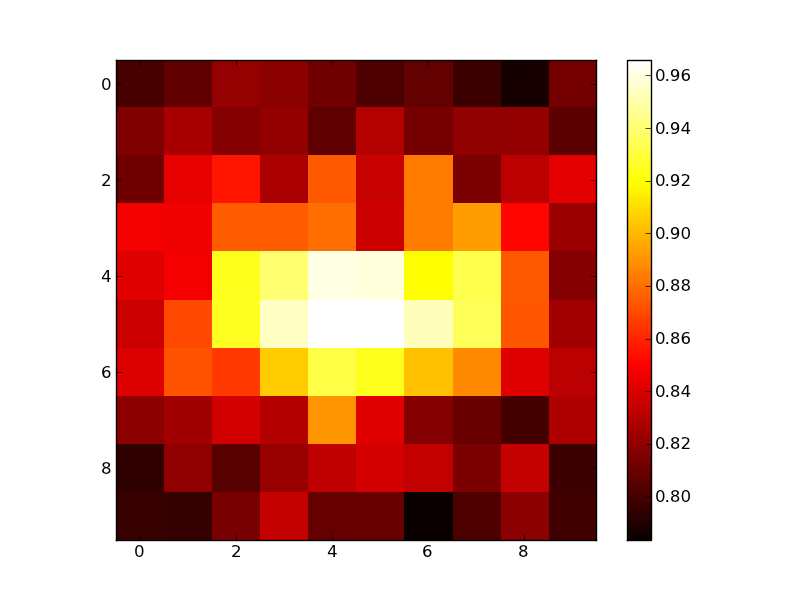
\includegraphics[width=.5\linewidth]{img/logistic_l1_scores.png}

\section{Encoding}

\alex{After talking with Michael, he told me that he could make a fairly simple
    example for encoding, which I think is a plus for the paper. The example will
    be integrated in Nisl.}




\section{Functional Connectivity}

In \cite{biswal1995}, Biswal was the first to exhibit coherent patterns in the
brain activation during resting state. These correlated voxel activations seemed
to form functional networks concording with neuroscientific knowledge.

Resting-state fMRI is useful when dealing with subjects that cannot execute a
specific task. For example, stroke patients suffer various brain disease that
are very difficult to diagnose; resting state fMRI may help by showing a
difference in the correlation between function brain networks.

As our data is unlabeled, we have to rely on unsupervised learning. The most
famous unsupervised method is the ICA and has been widely used to study resting
state data. We will also see how clustering algorithms behave on such data.

\subsection{Independent Component Analysis (ICA)}

\subsubsection{Intuition}

ICA is a blind source separation method. Its principle is to separate a
multivariate signal into several components by maximizing their non-gaussianity.
A typical example is the \emph{cocktail party problem} where ICA separates the
voices of people using signal from several mikes.

It is historically the reference method to extract networks from resting state
fMRI \cite{biswal1999}. Several strategies have been used to syndicate ICA
results across several subjects. \cite{calhoun2001a} proposes a dimension
reduction (using PCA) followed by a concatenation of the time series.
\cite{varoquaux2010} uses dimension reduction and canonical correlation analysis
to aggregate subject data.

\subsubsection{Application}

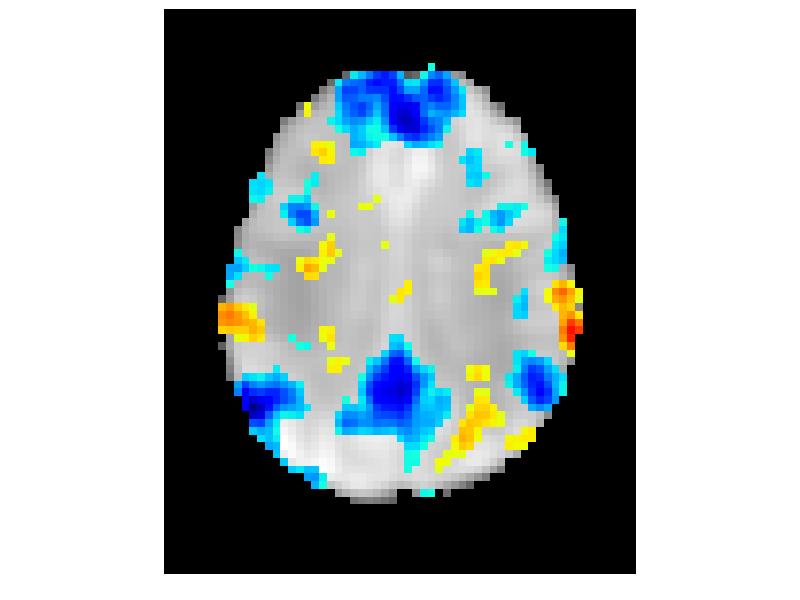
\includegraphics[width=.5\linewidth]{img/plot_canica_resting_state_17.png}

\subsection{Clustering}

Make  an  example  with   Ward   Clustering.  Indicate  then   that  other
algorithms  can  be  used  such  as
KMeans and Spectral clustering and only give results.

We use a PCA here to reduce dimensionality.

Bonus: may be used as dimensionality reduction


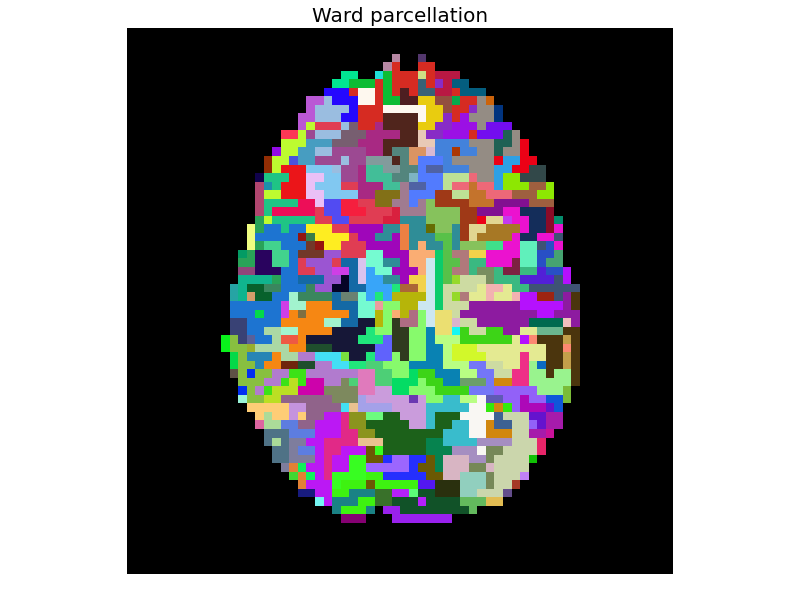
\includegraphics[width=.3\linewidth]{img/plot_rest_clustering_1.png}
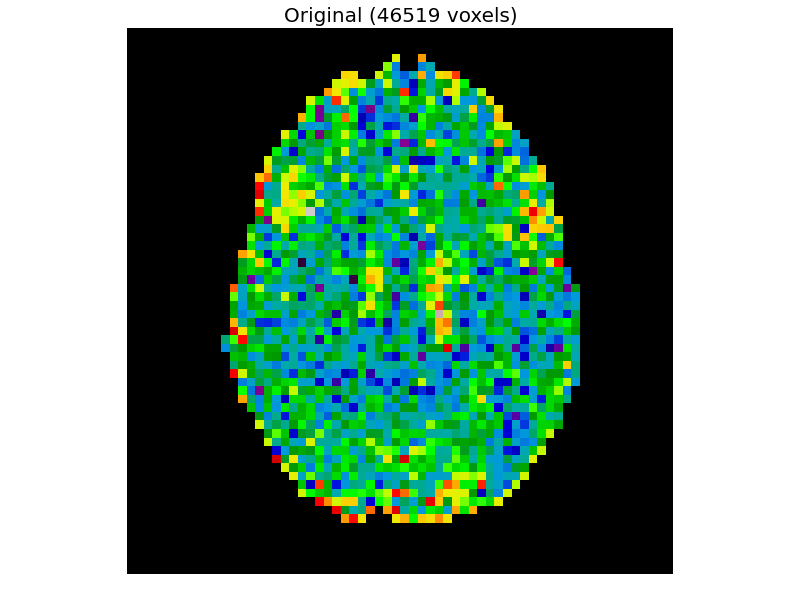
\includegraphics[width=.3\linewidth]{img/plot_rest_clustering_2.png}
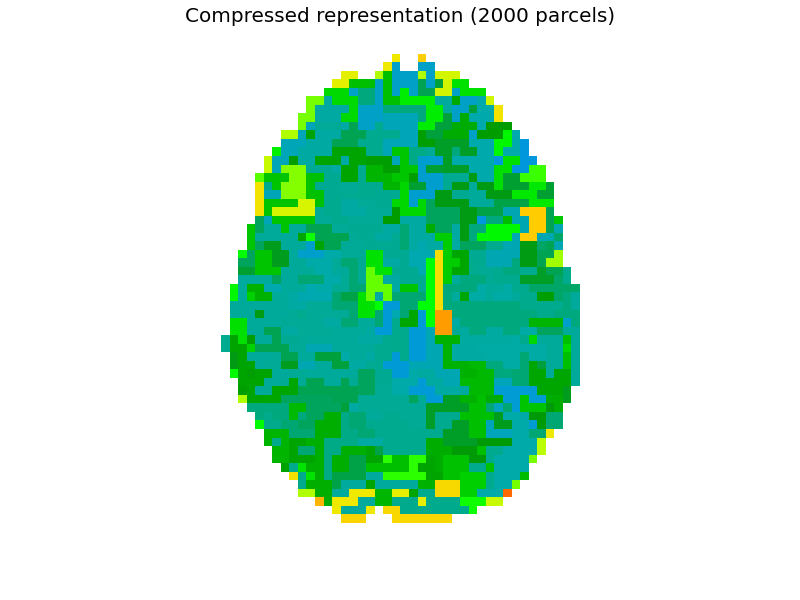
\includegraphics[width=.3\linewidth]{img/plot_rest_clustering_3.png}

\section*{Disclosure/Conflict-of-Interest Statement}
%All relationships financial, commercial or otherwise that might be perceived
%by the academic community as representing a potential conflict of interest
%must be described. If no such relationship exists, authors will be asked to
%declare that the research was conducted in the absence of any commercial or
%financial relationships that could be construed as a potential conflict of
%interest.
The authors declare that the research was conducted in the absence of any
commercial or financial relationships that could be construed as a potential
conflict of interest.

\section*{Acknowledgement} Text Text Text Text Text Text  Text Text Text Text
Text Text Text Text  Text Text Text Text Text Text Text Text Text  Text Text
Text.

\paragraph{Funding\textcolon} Text Text Text Text Text Text  Text Text.

\section*{Supplemental Data} Text Text Text Text Text Text  Text Text Text Text
Text Text Text Text Text  Text Text Text Text Text Text Text Text Text  Text
Text Text.

\bibliographystyle{frontiersinSCNS} % for Science articles
\bibliography{biblio}

\end{document}
